\documentclass{article}
\usepackage[utf8]{inputenc}

% Load a number of useful packages
\usepackage{graphicx}
\usepackage{amsmath,amssymb,amsfonts,amsthm}
 \usepackage[margin=1.0in]{geometry}
\usepackage[colorlinks=true]{hyperref}
\usepackage{cite}
\usepackage{float}

%\usepackage[caption=false,font=footnotesize]{subfig}


% Two more packages that make it easy to show MATLAB code
\usepackage[T1]{fontenc}
\usepackage[framed,numbered]{matlab-prettifier}
\lstset{
	style = Matlab-editor,
	basicstyle=\mlttfamily\small,
}
% Say where pictures (if any) will be placed
\graphicspath{ {./images/} }

%Define Title, author, date
\title{AE 353: Design Problem 04}
\author{Parthiv V Kukadia}
\date{6th December, 2020}

\begin{document}
\maketitle
This paper will describe the design, implementation, and testing of a controller for a 3D model of one of NASA’s Robonauts; similar to a segway robotic mobility platform \cite{RMP}. The Robonaut will attempt to race along randomly generated path in the least amount of time without crashing using the controller.

\section{Goal}
DesignProblem04 simulates a two-wheeled robot that is similar to the segway robotic mobility platform1, which has been considered for use with the NASA robonaut. The robonaut is equipped with actuators which allow me to specify the torque applied to each wheel. It also has sensors which allow me to measure the angular velocity of each wheel, the turning radius of a road along which the robot can drive, the error in lateral position, and the error in heading relative to this road. Multiple controllers will be designed to test out which controller is most effective in driving along a 120m long randomly generated road. The goal is to design a controller that will allow the robonaut to race along this road as fast as possible without crashing.

\section{Requirements and Verification}
Requirement for a successful controller: 80$\%$ finish rate racing on 5 randomly generated roads in under 60s.\\
\\
Verification will be done via the MATLAB DesignProblem04 simulator. The controllers will be run through 5 randomly generated roads and they will have to complete the track successfully. The results will be tabulated and displayed. If the controller has 4 finishes out of the 5 races in under 60 s, the controller will have met the requirement.

\section{Model}
\subsection{Variables}
This section provides information about how variables are named in \lstinline{DesignProblem04}. The equations of motion are used to establish the motion of the robonaut. The variables to the equations of motion are:
\begin{itemize}
\item $\phi$, the chassis angle, phi
\item $\dot{\phi}$, the time derivative of the chassis angle, phidot
\item $v$, the forward speed, v
\item $w$, the turning rate, w
\item $\tau_{R}$ and $\tau_{L}$, the right and left motor torques, tauR and tauL
\end{itemize}
These variables were initialized in Matlab as symbolic variables using \lstinline{syms}.\\
There are two extra equations of motion, and the variables to these equations are:
\begin{itemize}
\item $e_\text{lateral}$, the lateral error in following the road, elateral
\item $e_\text{heading}$, the heading error in following the road, eheading
\item $w_\text{road}$ the turning rate of a trajectory that would follow the road centerline, wroad
\item $v_\text{road}$ the forward speed of a trajectory that would follow the road centerline,  vroad
\end{itemize}

These variables were also initialized using \lstinline{syms}. It should be brought to readers attention that $v_\text{road}$ and $w_\text{road}$ are not states, they are parameters that the model depends on. 

\subsection{Robonaut}
The motion of the robonaut is governed by the second order ordinary differential equations with the form
\begin{equation}
\label{eqEOM}
\begin{bmatrix} \ddot{\phi} \\ \dot{v} \\ \dot{w} \end{bmatrix} = f(\phi,\dot{\phi},v,w,\tau_{R},\tau_{L})
\end{equation}
where $\phi$ is the pitch angle of the chassis, $\dot{\phi}$ is the pitch angular velocity, $v$ is the forward
speed, $w$ is the turning rate, and $\Tau_{R}$ and $\Tau_{L}$ are the torques applied by the chassis to the right
and left wheel, respectively.\\
\\
For the purpose of my control design to follow a road, it is useful to keep track of the position and orientation relative to the road as opposed to an absolute reference frame. The sensors can report the radius of curvature $r_\text{road}$ of the road along which the robot is currently moving (where $r_\text{road}<0$ instructs the robonaut to turn right, $r_\text{road}<0$ instructs the robonaut to turn left, $r_\text{road}=0$ instructs the robonaut to turn in its place to re-orient itself, and $r_\text{road}=\infty$ instructs the robonaut to go straight). Knowing a speed, $v_\text{road}$, at which the robot can travel along the road, the turning rate $w_\text{road}$ necessary to follow the centerline can be computed as
\begin{equation}
\label{eqncurv}
w_\text{road} = \frac{v_\text{road}}{r_\text{road}}.
\end{equation}

Two more equations are useful to me:
\begin{align}
\dot{e}_\text{lateral} &= -v\sin\left(e_\text{heading}\right) \label{eqnLat}\\
\dot{e}_\text{heading} &= w-\left(\frac{v\cos\left(e_\text{heading}\right)}{v_\text{road}+w_\text{road}e_\text{lateral}}\right)w_\text{road} \label{eqnHead}
\end{align}
where $e_{lateral}$ is the perpendicular distance from the centerline of the road to the
position $(x;y)$ of the robot (where $e_{lateral}$ > 0 means being too far to the right and $e_{lateral}$ < 0
means being too far to the left), and $e_{heading}$ is the difference between the orientation
$\theta$ of the robot and the direction of the road.\\

\par
The linear state space model is represented by two equations:
\begin{align}
\dot{x} &= Ax + Bu \label{eqnState}\\
y &= Cx + Du \label{eqnOutput}
\end{align}

In this design problem, there is no feed-forward so the $D$ matrix in Eq.\eqref{eqnOutput} is $D = [0]$. The EOM's are used to define the state, $x$, and input, $u$. The robonaut's sensors provide the information to form the output, $y$, with the following derived relationships between the angular velocity of the robonaut's wheels, speed, and turning rate:
\begin{align}
w_{R} & = \frac{1}{r}v + \frac{b}{2r}w  & 
w_{L} & = \frac{1}{r}v - \frac{b}{2r}w 
\end{align}
\\
Therefore to begin linearizing the non-linear equations of motion, we chose an equilibrium point. The function $f$ in Eq. \eqref{eqEOM} was run through DesignProblem04 and stored in a data.mat file symbolically. The state variables of interest, input vector, and output vector are defined from the variables of the parsed EOMs, and an initial guess was made about the values of these variables to determine the equilibrium points.
\begin{equation}
\label{eqnState}
x=
\begin{bmatrix}
\phi - \phi_{\text{e}}\\
\dot{\phi} - \dot{\phi}_{\text{e}}\\
v - v_{\text{e}}\\
w- w_{\text{e}}\\
e_\text{lateral} - e_\text{lateral-e} \\
e_\text{heading} - e_\text{heading-e}\\
\end{bmatrix} \qquad
u =
\begin{bmatrix}
\tau_{R} - \tau_{R-\text{e}}\\
\tau_{L} - \tau_{L-\text{e}}\\
\end{bmatrix} \qquad
y =
\begin{bmatrix}
w_{R} - w_{R-\text{e}}\\
w_{L} - w_{L-\text{e}}\\
e_\text{lateral} - e_\text{lateral-e} \\
e_\text{heading} - e_\text{heading-e}\\
\end{bmatrix}
\end{equation}
\begin{equation*}
x_{equilibrium} =
\begin{bmatrix} 
0\\0\\6\\0\\0\\0
\end{bmatrix}\qquuad \qquad
u_{equilibrium} =
\begin{bmatrix}
0\\0
\end{bmatrix}
\end{equation*}
\par
The chosen values for equilibrium in Eq.(\eqref{eqnState}) were such that there would be no movement away from the center line, so that the robonaut would move in a straight line whilst remaining upright. As the robonaut is moving forward, $v_{\text{e}}$ can be a varying positive number, so I chose an arbitrary value. All other values were set to 0 to allow a forward moving straight line motion.
\par
 The equilibrium values were then used in the Jacobian function to produce state space matrices $A$, $B$, and $C$. These matrices were computed as partial derivatives of $f$ and $y$ with respect to $x$ and $u$ evaluated around the equilibrium points. The matrices are represented by
\begin{align}
A = \frac{\partial f}{\partial x}\biggr\rvert_{(x_{\text{e}}, u_{\text{e}})} \qquad
B = \frac{\partial f}{\partial u}\biggr\rvert_{(x_{\text{e}}, u_{\text{e}})}  \qquad
C = \frac{\partial y}{\partial x}\biggr\rvert_{(x_{\text{e}}, u_{\text{e}})} 
\end{align}
Providing me with the following state space matrices:
\begin{equation*}
   A = \begin{bmatrix}
    0 & 1 & 0 & 0 & 0 & 0\\
    27.4427 & 0 & 0 & 0 & 0 & 0\\
    -3.4540 & 0 & 0 & 0 & 0 & 0\\
    0 & 0 & 0 & 0 & 0 & 0\\
    0 & 0 & 0 & 0 & 0 & -6\\
    0 & 0 & 0 & 1 & 0 & 0
    \end{bmatrix} \qquad B = \begin{bmatrix}
    0 & 0\\ -2.2255 &  -2.2255\\
    0.5874  &  0.5874\\
    2.4814  & -2.4814\\ 0& 0\\ 0 & 0
    \end{bmatrix}\\ 
\end{equation*}
\begin{equation*}
    C = \begin{bmatrix}
0& 0& 5&1& 0&  0\\
0&0& 5& -1&0& 0\\
0& 0& 0& 0& 1&  0\\
0& 0& 0& 0& 0&  1
\end{bmatrix} \qquad 
D = 
\begin{bmatrix}
    0
\end{bmatrix}\\
\end{equation*}

This provides us with the following state space equations:
\begin{equation*}
\begin{bmatrix}
\dot{phi}\\
\ddot{\phi}\\
\dot{v}\\
\dot{w}\\
\dot{e_\text{lateral}}\\
\dot{e_\text{heading}}
\end{bmatrix} \qquad
=
\begin{bmatrix}
0 & 1 & 0 & 0 & 0 & 0\\
    27.4427 & 0 & 0 & 0 & 0 & 0\\
    -3.4540 & 0 & 0 & 0 & 0 & 0\\
    0 & 0 & 0 & 0 & 0 & 0\\
    0 & 0 & 0 & 0 & 0 & -6\\
    0 & 0 & 0 & 1 & 0 & 0
\end{bmatrix}
\begin{bmatrix} 
\phi \\
\dot{\phi}\\
v\\
w\\
e_\text{lateral} \\
e_\text{heading}
\end{bmatrix}
+
\begin{bmatrix}
 0 & 0\\ -2.2255 &  -2.2255\\
    0.5874  &  0.5874\\
    2.4814  & -2.4814\\ 0& 0\\ 0 & 0
    \end{bmatrix}
    \begin{bmatrix}
    \tau_{R}\\
\tau_{L}
    \end{bmatrix}
\end{equation*}
and output
\begin{equation*}
y =
\begin{bmatrix}
w_{R}\\
w_{L}\\
e_\text{lateral}\\
e_\text{heading}
\end{bmatrix}
=
\begin{bmatrix}
0& 0& 5&1& 0&  0\\
0&0& 5& -1&0& 0\\
0& 0& 0& 0& 1&  0\\
0& 0& 0& 0& 0&  1
\end{bmatrix}
\begin{bmatrix}
\phi \\
\dot{\phi}\\
v\\
w\\
e_\text{lateral} \\
e_\text{heading}
\end{bmatrix}
+
\begin{bmatrix} 
0
\end{bmatrix}
\begin{bmatrix}
    \tau_{R}\\
\tau_{L}
    \end{bmatrix}
\end{equation*}
Now that we have the state space matrices, we can check for controllability, which is given from the matrix W. A system is controllable when the rank of matrix W = the length of matrix A, which in this case, it does, and it = 6. Length(A) = rank(W) = 6.\\
Despite the system being controllable, it's asymptotically unstable. This means that the real eigenvalues of A are not all negative. Since that is the case, it is highly likely that the robonaut will either crash or go off. the road. Therefore, we must design a controller that will allow us to improve our controller.
\begin{equation*}
    eig(A) = \begin{bmatrix}
    0\\5.2386\\-5.2386\\0\\0\\0
    \end{bmatrix}
\end{equation*}
We can go on to check if our system is observable or not now. This is done using the MATLAB function obsv(A,C), and we compare the rank of this O matrix with length of the A matrix, which are both 6. Therefore we can say that our system is observable. Length(A) = rank(O) = 6.
\section{Control Design}
This section has been written out, but matrices are not confirmed as of now. They will change depending on how the controller works.
\subsection{Controllability}
To design the controller, the system needs to be controllable. We need to check for controllability as it allows system to move via the input from an intial state to the final state. We found controllability above. Therefore, we know go on to find the controller gain matrix, $K$, which can be found using the lqr function in MATLAB, using state cost weighted matrix and input cost weighted matrix. \\
\begin{equation}
    K = lqr(A,B,Q_{c},R_{c})
\end{equation}
The cost weighted matrices used were;
\begin{equation*}
    Q_{c} = \begin{bmatrix}
    1 & 0 & 0 & 0 & 0& 0\\
    0 & 1 & 0 & 0 & 0 & 0\\
    0 & 0 & 1 & 0 & 0 & 0\\
    0 & 0 & 0 & 1 & 0& 0\\
    0 & 0 & 0 & 0 & 450000& 0\\0&0&0&0&0&450000
    \end{bmatrix} , R_{c} = \begin{bmatrix}
    10
    \end{bmatrix}
\end{equation*}
This outputted a K matrix of;
\begin{equation}
    K = \begin{bmatrix}
-12.6635 & -2.4556 & -0.2236 & 8.8959 & -150.0000 & 196.2465\\
-12.6635 & -2.4556 & -0.2236 & -8.8959 & 150.0000 & -196.2465
    \end{bmatrix}
\end{equation}

\subsection{Observability}
In my case, as I don't have complete knowledge of the state, a new ODE is formed, where I require L as shown below:
\begin{equation}
    \hat{\dot{x}} = A\hat{x} + Bu - L(C\hat{x} - y)
\end{equation} \cite{Astrom2010}
Where L, the observer gain matrix is formed using:
\begin{equation}
    L = lqr(A',C',inv(R_{o}),inv(Q_{o}))'
\end{equation}
With the observer matrices being:
\begin{equation*}
    R_{o}= \begin{bmatrix}
     1 & 0 & 0 & 0 & 0& 0\\
    0 & 1 & 0 & 0 & 0 & 0\\
    0 & 0 & 1 & 0 & 0 & 0\\
    0 & 0 & 0 & 1 & 0& 0\\
    0 & 0 & 0 & 0 & 5& 0\\0&0&0&0&0&5
    \end{bmatrix} , Q_{o} = \begin{bmatrix}
    30
    \end{bmatrix}
\end{equation*}
Outputting a L matrix of:
\begin{equation}
    L = \begin{bmatrix}
    -13.9784 & -13.9784 & -0.0000   & 0.0000\\
    -70.4667 & -70.4667 &  -0.0000 &   0.0000\\
   4.9655  &  4.9655   & 0.0000 & -0.0000\\
  3.8626 &  -3.8626 &  -0.1297 &   0.3786\\
    -0.1297 & 0.1297   & 4.8402 &  -1.6943\\
    0.3786 &  -0.3786  & -1.6943 &   1.8973
    \end{bmatrix}
\end{equation}

\subsection{Stability}
We then go on to make 2 final checks regarding the asymptotic stability of the system. If they have all negative real parts, then the system is stable.
\begin{equation*}
    eig(A-BK) = \begin{bmatrix}
-0.1372 + 0.0000i\\
  -4.7723 + 0.0000i\\
  -5.7577 + 0.0000i\\
 -19.0776 +19.5268i\\
 -19.0776 -19.5268i\\
  -5.9933 + 0.0000i\\
    \end{bmatrix} \qquad eig(A-CL) = \begin{bmatrix}
-38.5684 + 0.0000i\\
  -7.2619 + 0.0000i\\
  -3.8248 + 0.0000i\\
  -7.7349 + 0.0000i\\
  -3.3639 + 2.2870i\\
  -3.3639 - 2.2870i\\
    \end{bmatrix}
\end{equation*}
The results that we obtain show that our system is now asymptotically stable; will tend to zero, allowing me to implement and test my controller.

\section{Testing}
Having successfully verified controllability and observability, we can now implement our controller into the system. I made 3 controllers, with varying gains. The first controller has high speed, as well as a high turning rate, and a high chassis angle. The second one is adjusted and has controller gain matrices that have the same values. The last controller has a slower speed and gain matrices where $R_{c}$ is much smaller than $Q_{c}$. The three controllers and the reasoning behind the changes will be spoken about in this section. When creating the controllers, many errors came into play. This meant that the controller crashed, and there were only 2 reasons why the controller would crash, either it drove off the road, or it tipped over. The issue of crashing could be de-bugged by changing w (if robot was turning into a crash) or $\phi$ (if robot was tipping). $e_{lateral}$ and $e_{heading}$ were focused on in the gain matrix if the robot was veering off the road.\\
Regardless of these tweaks, I should mention that failure occured most often on roads that had consecutive sharp turns, and the controller was unable to recover and stabilize in time. The controller was able to stabilize in time if it was one sharp turn, but did not have enough time to stabilize with them being back to back.

\subsection{Controller 1}
This controller is the original controller, with high velocity with equilibrium velocity being 6 m/s and gains as shown below:

\begin{equation*}
    Q_{c} = \begin{bmatrix}
    1 & 0 & 0 & 0 & 0& 0\\
    0 & 1 & 0 & 0 & 0 & 0\\
    0 & 0 & 1 & 0 & 0 & 0\\
    0 & 0 & 0 & 1 & 0& 0\\
    0 & 0 & 0 & 0 & 450000& 0\\0&0&0&0&0&450000
    \end{bmatrix} , R_{c} = \begin{bmatrix}
    10
    \end{bmatrix}
\end{equation*}
and observer gain being:
 \begin{equation*}
     R_{o}= \begin{bmatrix}
     1 & 0 & 0 & 0 & 0& 0\\
    0 & 1 & 0 & 0 & 0 & 0\\
    0 & 0 & 1 & 0 & 0 & 0\\
    0 & 0 & 0 & 1 & 0& 0\\
    0 & 0 & 0 & 0 & 5& 0\\0&0&0&0&0&5
    \end{bmatrix} , Q_{o} = \begin{bmatrix}
    30
    \end{bmatrix}
 \end{equation*}
 This controller was able to operate well, but had a success rate of only 60 percent, as it was unsuccessful in making consecutive sharp turns.
 \begin{figure}[H]
\centering
\begin{minipage}{.5\textwidth}
	\centering
	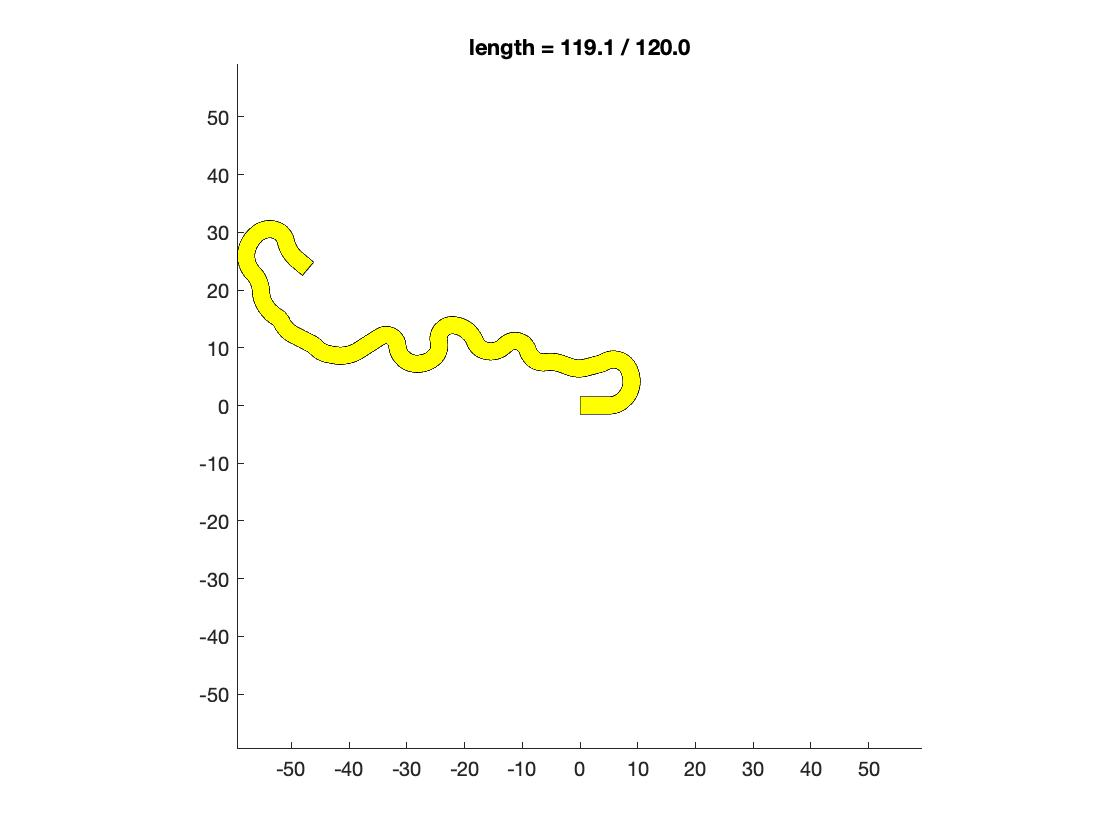
\includegraphics[width=.8\linewidth]{failure 2 track.jpg}
	\caption{Failure Track}
	\end{minipage}%
\begin{minipage}{.5\textwidth}
	\centering
	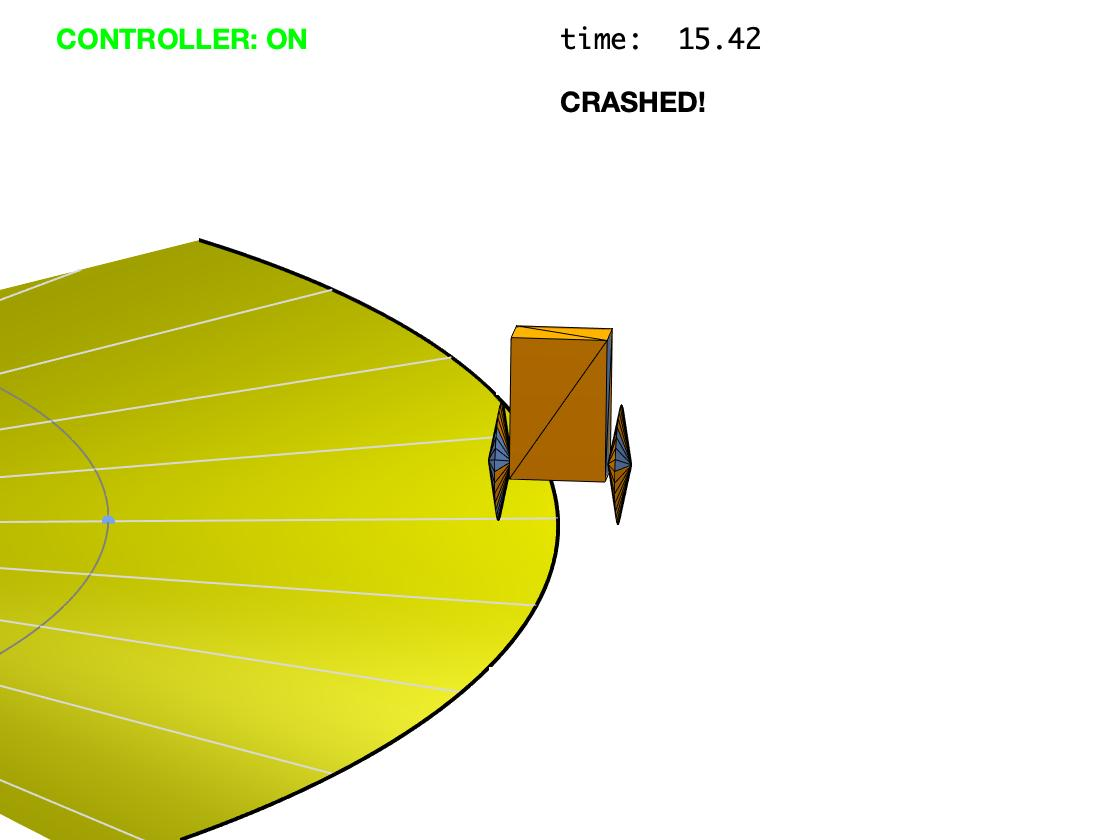
\includegraphics[width=.8\linewidth]{failure 2 robot.jpg}
	\caption{Robonaut Crash}
\end{minipage}
\end{figure}
As we can see in the figure above, the robonaut veers off the track where there are multiple turns. The robonaut went off track as too much leeway was given to it in the observer matrix, allowing it to move away from the centerline by a larger amount. This means that $R_{o}$ needs to reduce to make sure that the turn isn't as loose. Another reason that this controller didn't work was because of the velocity. The robonaut was travelling too fast for it to stabilize in time during these turns and re-align itself with the center-line, causing it to veer off track, and crashing. Therefore, to eliminate this kind of failure, I reduced the speed of the robonaut, and further reduced the leeway allowed in my observer matrices. As the robot veered off the track, that means that I need to change my $e_{lateral}$ and $e_{heading}$ in my controller matrix to get my robonaut to stay closer to the center-line.
\subsection{Controller 2}
This controller was adjusted from the original controller, with a lower velocity being 5.8 m/s, and a change in the controller and observer matrices at $e_lateral$ and $e_{heading}$, to adjust for the veering off, and allowing it time to re-stabilize itself. The gains are shown below:

\begin{equation*}
    Q_{c} = \begin{bmatrix}
    1 & 0 & 0 & 0 & 0& 0\\
    0 & 1 & 0 & 0 & 0 & 0\\
    0 & 0 & 1 & 0 & 0 & 0\\
    0 & 0 & 0 & 1 & 0& 0\\
    0 & 0 & 0 & 0 & 470000& 0\\0&0&0&0&0&470000
    \end{bmatrix} , R_{c} = \begin{bmatrix}
    10
    \end{bmatrix}
\end{equation*}
and observer gain being:
 \begin{equation*}
     R_{o}= \begin{bmatrix}
     1 & 0 & 0 & 0 & 0& 0\\
    0 & 1 & 0 & 0 & 0 & 0\\
    0 & 0 & 1 & 0 & 0 & 0\\
    0 & 0 & 0 & 1 & 0& 0\\
    0 & 0 & 0 & 0 & 4.8& 0\\0&0&0&0&0&4.8
    \end{bmatrix} , Q_{o} = \begin{bmatrix}
    30
    \end{bmatrix}
 \end{equation*}
 Therefore testing this controller on a track with sharp turns, we see that the controller is able to make those turns, whilst being able to re-stabilize itself and keep itself inbounds. 
 \begin{figure}[H]
\centering
\begin{minipage}{.5\textwidth}
	\centering
	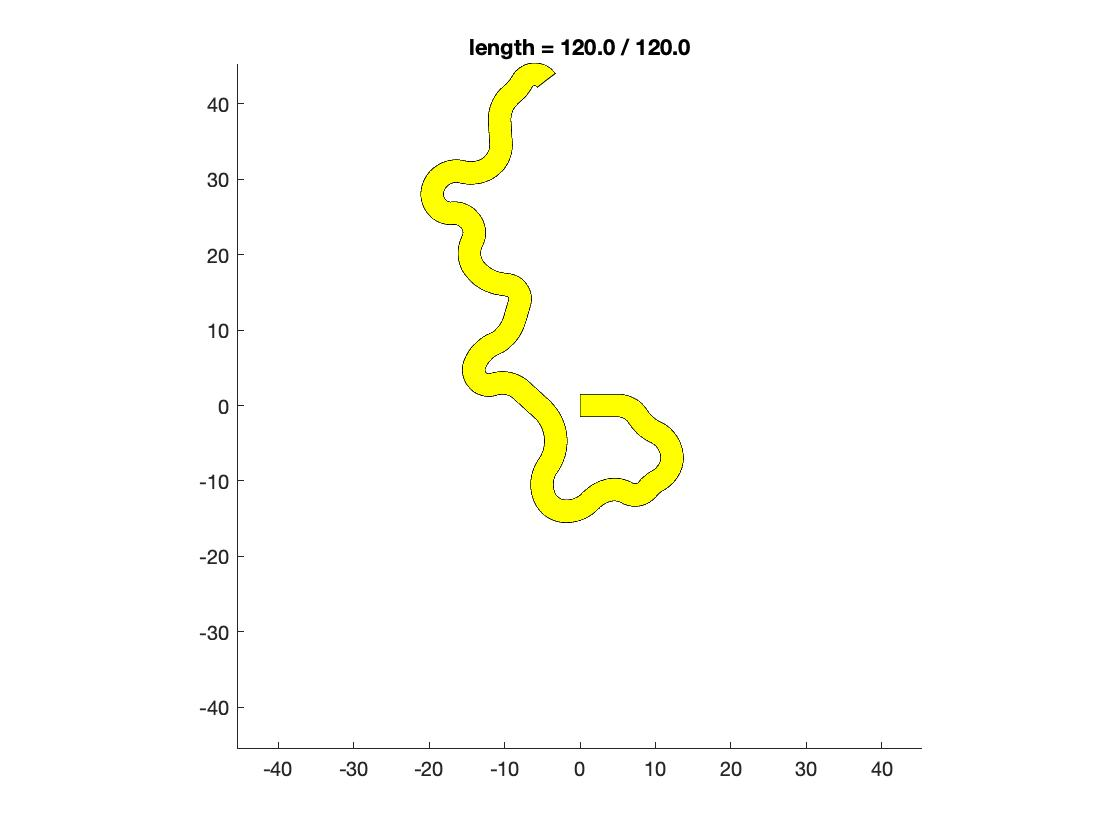
\includegraphics[width=.8\linewidth]{failure eliminated track.jpg}
	\caption{Failure Eliminated Track}
	\end{minipage}%
\begin{minipage}{.5\textwidth}
	\centering
	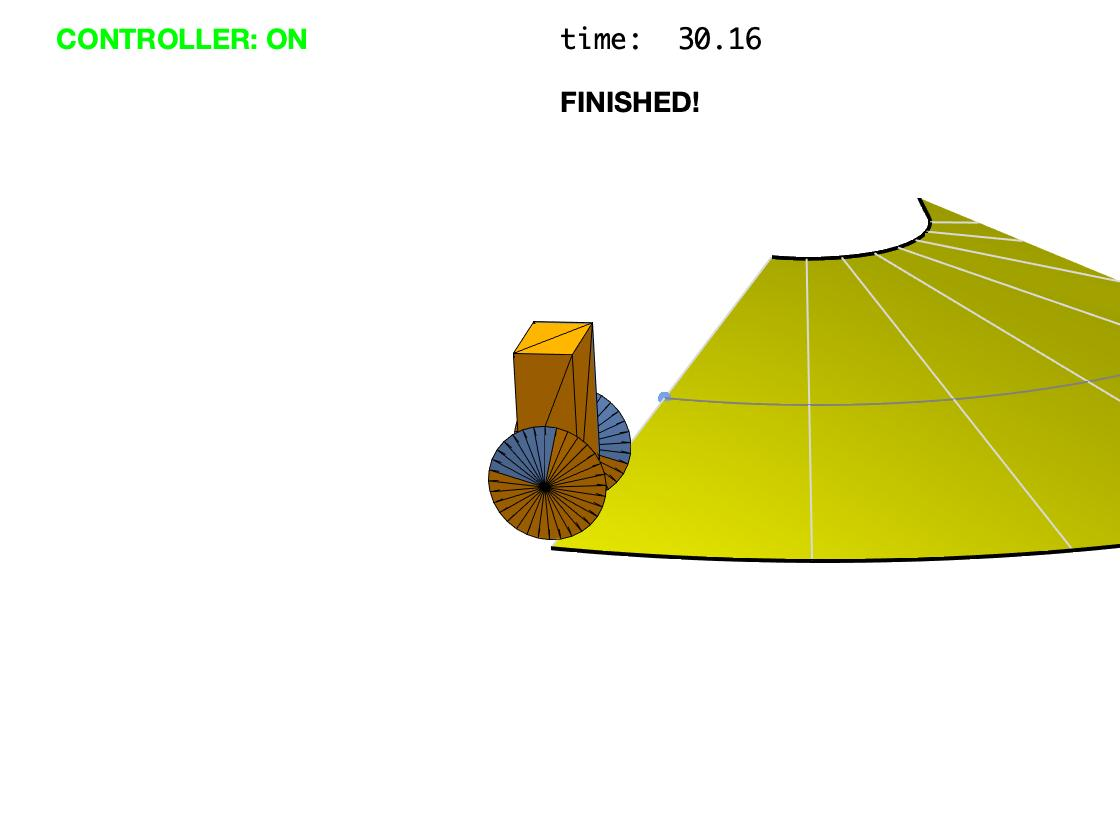
\includegraphics[width=.8\linewidth]{Failure eliminated.jpg}
	\caption{Robonaut Success}
\end{minipage}
\end{figure}
As we can see, the track had several consecutive sharp turns, but the robonaut successfully managed to complete it. This means that we managed to eliminate the issue of the robonaut veering off by changing $e_lateral$ and $e_{heading}$ as well as the velocity. However, the robonaut takes 30 seconds to complete the track, which completes the requirement set forward in terms of time, but I would like it to be quicker, so I changed the velocity back to 6 m/s to see if it possible for the robonaut to achieve success. The reason I want the robonaut to go faster is that with a faster robonaut, it would allow me to be a good racer in the competition, and so I increase the speed, and test the controller 5 times on 5 random roads to see if it has a 80$\%$ success rate.\\
Testing it on 5 random roads, we obtain the following:
\begin{table}[h!]
\centering
\begin{tabular}{|p{4cm}|p{4cm}|p{4cm}|}
\hline
Road & Time (sec)\\
\hline \hline
Road 1 & 27.58\\
Road 2 & 28.28\\
Road 3 & 27.60\\ 
Road 4 & 28.02\\ 
Road 5 & Crashed\\
\hline
\end{tabular}
\caption{Road Completion Times\label{roadTimesGain}}
\end{table}
Therefore, we managed to achieve the 80 $\%$ success rate, but there was a failure in the last track, shown below:
 \begin{figure}[H]
\centering
\begin{minipage}{.5\textwidth}
	\centering
	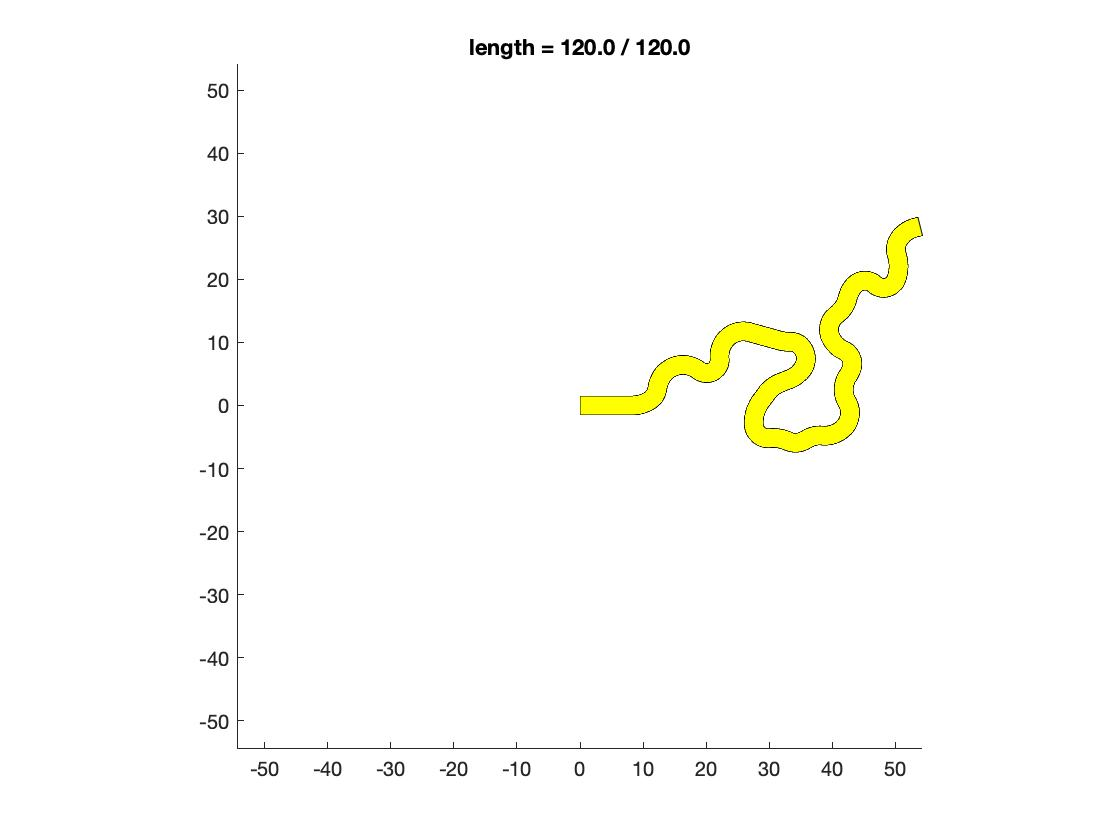
\includegraphics[width=.8\linewidth]{controller 2 failure.jpg}
	\caption{Failure Track}
	\end{minipage}%
\begin{minipage}{.5\textwidth}
	\centering
	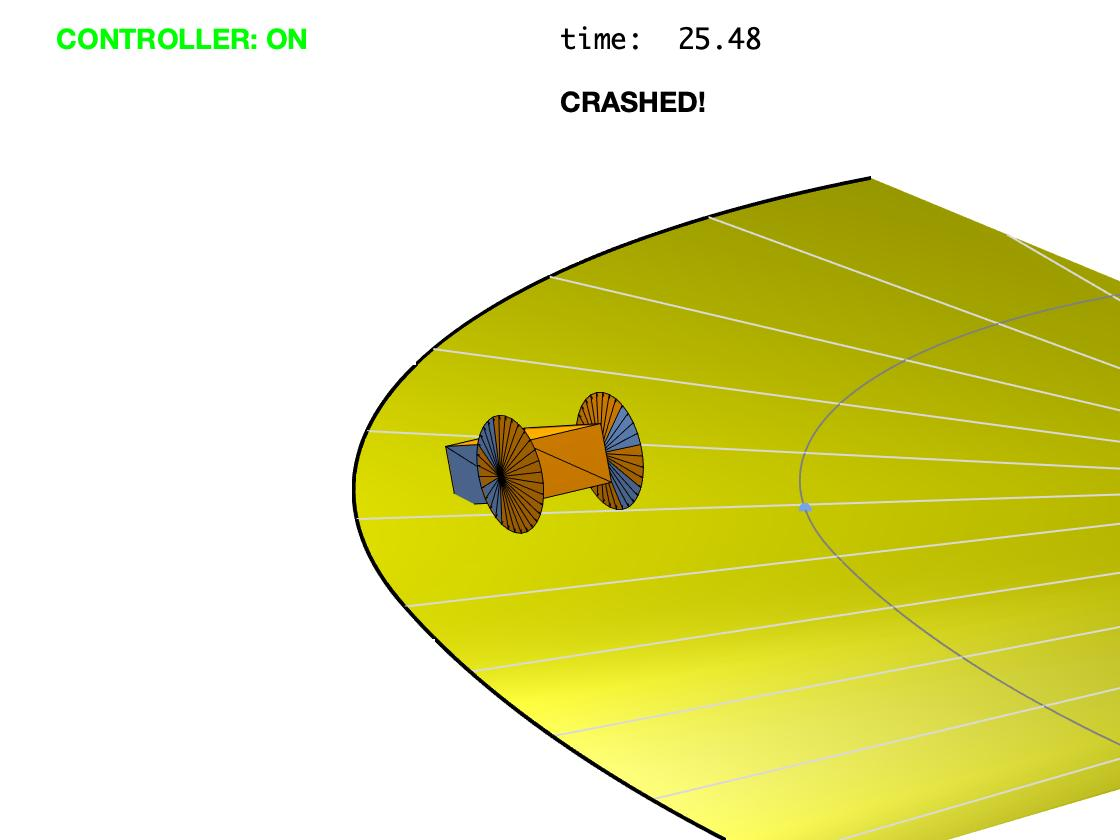
\includegraphics[width=.8\linewidth]{controller 2 fail.jpg}
	\caption{Robonaut Failure}
\end{minipage}
\end{figure}
We can see that the controller was working quite efficiently and was near the finish line when it crashed. This time, the crash wasn't it veering off the track, but it tipped over on the last turn. This means that I need to adjust my w and $\phi$ in my controller gains matrix to account for that crash. The reason this happened was because despite keeping my robonaut closer to the line, it tried to turn re-adjust too fast, causing it to loose balance and topple over. Therefore, I take that into account and increase my chassis angle and decrease my turning rate.
\subsection{Controller 3}
This controller was adjusted from controller 2, with a lower equilibrium velocity of 5.8 m/s, and a change in the controller and observer matrices at $\phi$ and w, to adjust for the tipping and crashing. This should allow my controller to re-stabilize itself after turns, and not crash. However, after nearly 100 different iterations, I changed a lot more than those 2 values, providing me with a fast, and efficient controller with the gains shown below:
\begin{equation*}
    Q_{c} = \begin{bmatrix}
    65 & 0 & 0 & 0 & 0& 0\\
    0 & 8.5 & 0 & 0 & 0 & 0\\
    0 & 0 & 8.5 & 0 & 0 & 0\\
    0 & 0 & 0 & 9 & 0& 0\\
    0 & 0 & 0 & 0 & 490000& 0\\0&0&0&0&0&490000
    \end{bmatrix} , R_{c} = \begin{bmatrix}
    10
    \end{bmatrix}
\end{equation*}
and observer gain being:
 \begin{equation*}
     R_{o}= \begin{bmatrix}
     1 & 0 & 0 & 0 & 0& 0\\
    0 & 1 & 0 & 0 & 0 & 0\\
    0 & 0 & 1 & 0 & 0 & 0\\
    0 & 0 & 0 & 1 & 0& 0\\
    0 & 0 & 0 & 0 & 5& 0\\0&0&0&0&0&5
    \end{bmatrix} , Q_{o} = \begin{bmatrix}
    30
    \end{bmatrix}
 \end{equation*}
 These gains were implemented into 5 consecutively randomly generated roads, and the results are shown below:
 \begin{table}[h!]
\centering
\begin{tabular}{|p{4cm}|p{4cm}|p{4cm}|}
\hline
Road & Time (sec)\\
\hline \hline
Road 1 & 25.70\\
Road 2 & 25.46\\
Road 3 & 25.84\\ 
Road 4 & 25.24\\ 
Road 5 & 25.58\\
\hline
\end{tabular}
\caption{Road Completion Times\label{roadTimesGain}}
\end{table}
When playing around with the values, there was a gains combination that allowed me to average 24s a track, but it also failed the 5th run, thus the gains was changed to the final controller 3 gains shown above. The randomly generated tracks and controller 3's successes are shown below:
\begin{figure}[H]
\centering
\begin{minipage}{.5\textwidth}
	\centering
	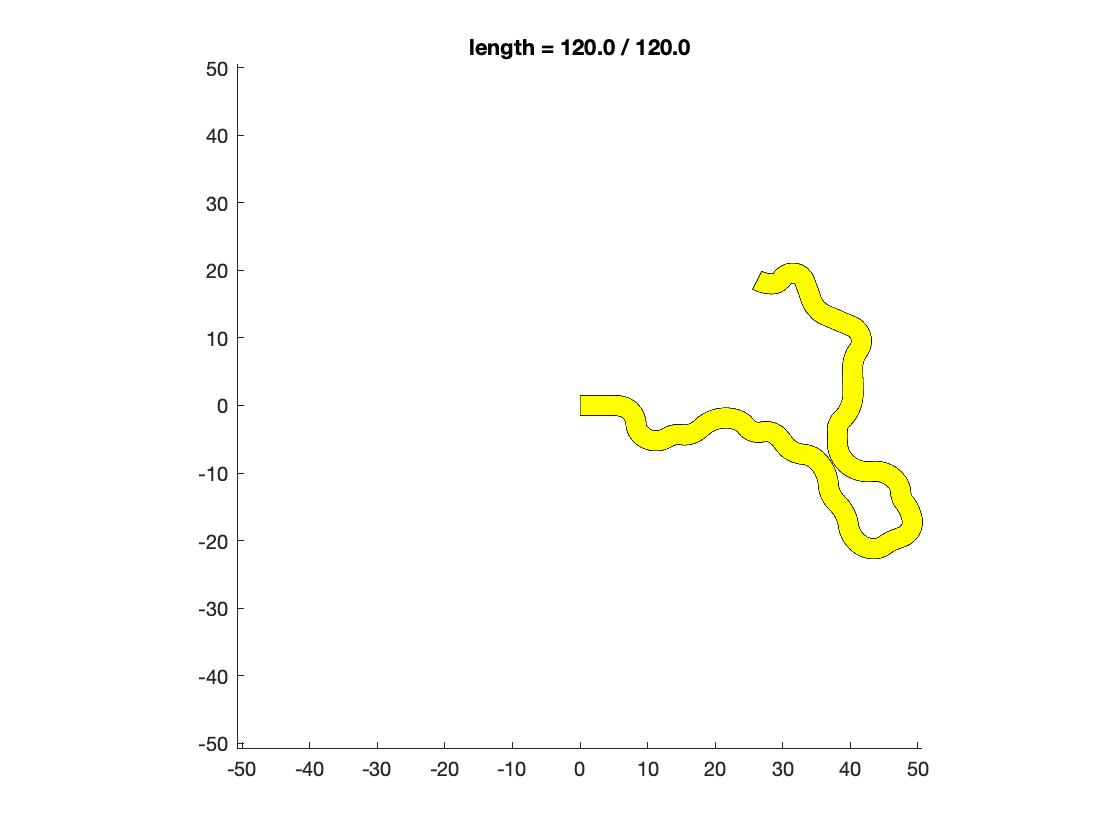
\includegraphics[width=.8\linewidth]{track 1.jpg}
	\caption{Track 1}
	\end{minipage}%
\begin{minipage}{.5\textwidth}
	\centering
	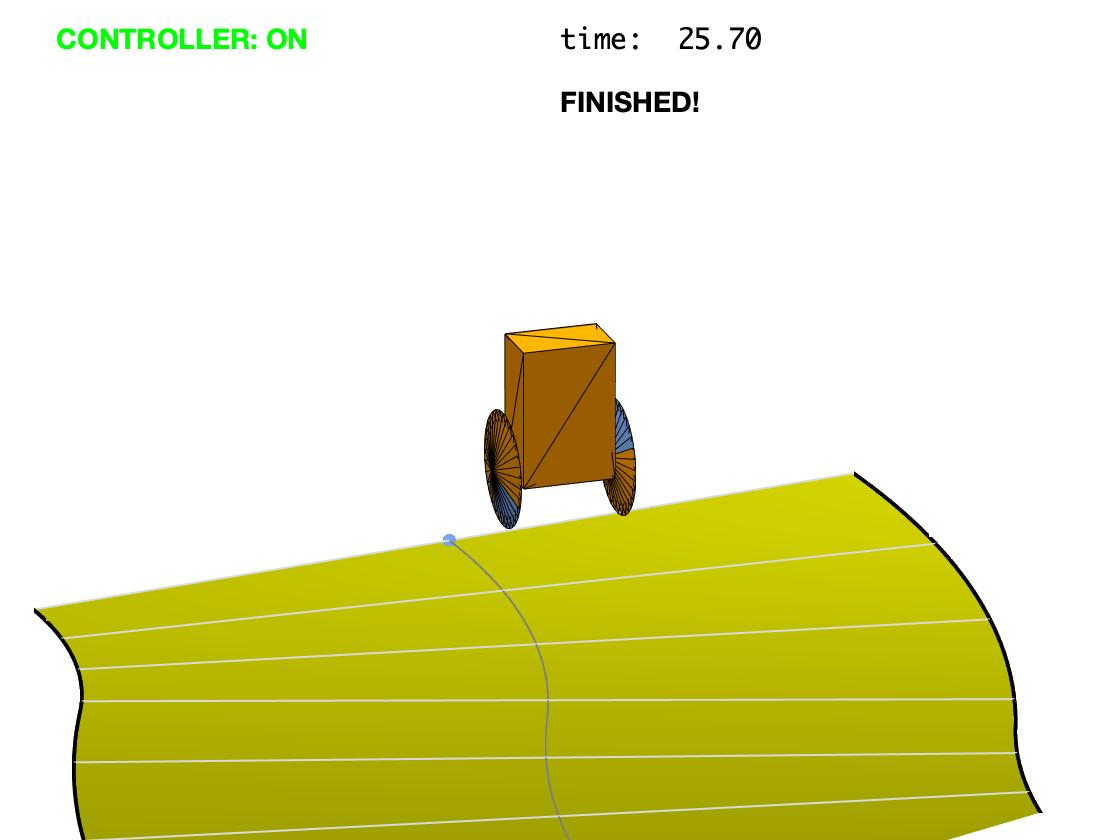
\includegraphics[width=.8\linewidth]{track 1r.jpg}
	\caption{Success 1}
\end{minipage}
\end{figure}
\begin{figure}[H]
\centering
\begin{minipage}{.5\textwidth}
	\centering
	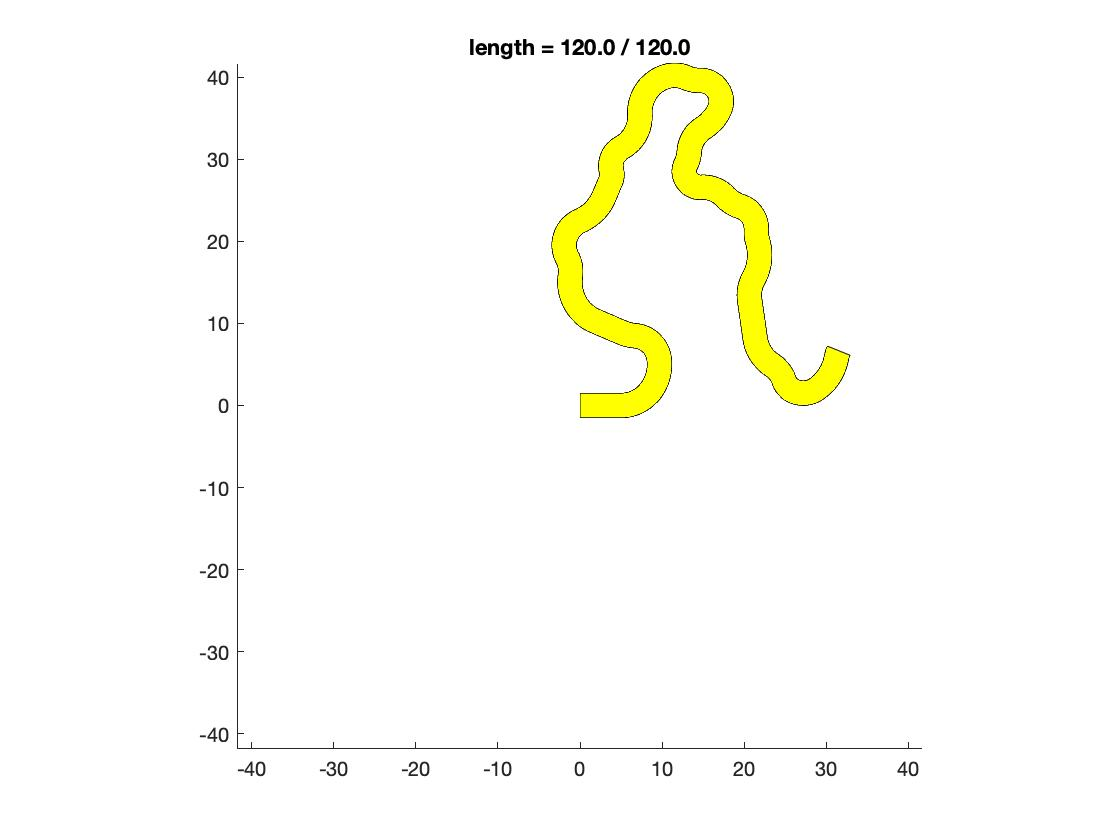
\includegraphics[width=.8\linewidth]{track 2.jpg}
	\caption{Track 2}
	\end{minipage}%
\begin{minipage}{.5\textwidth}
	\centering
	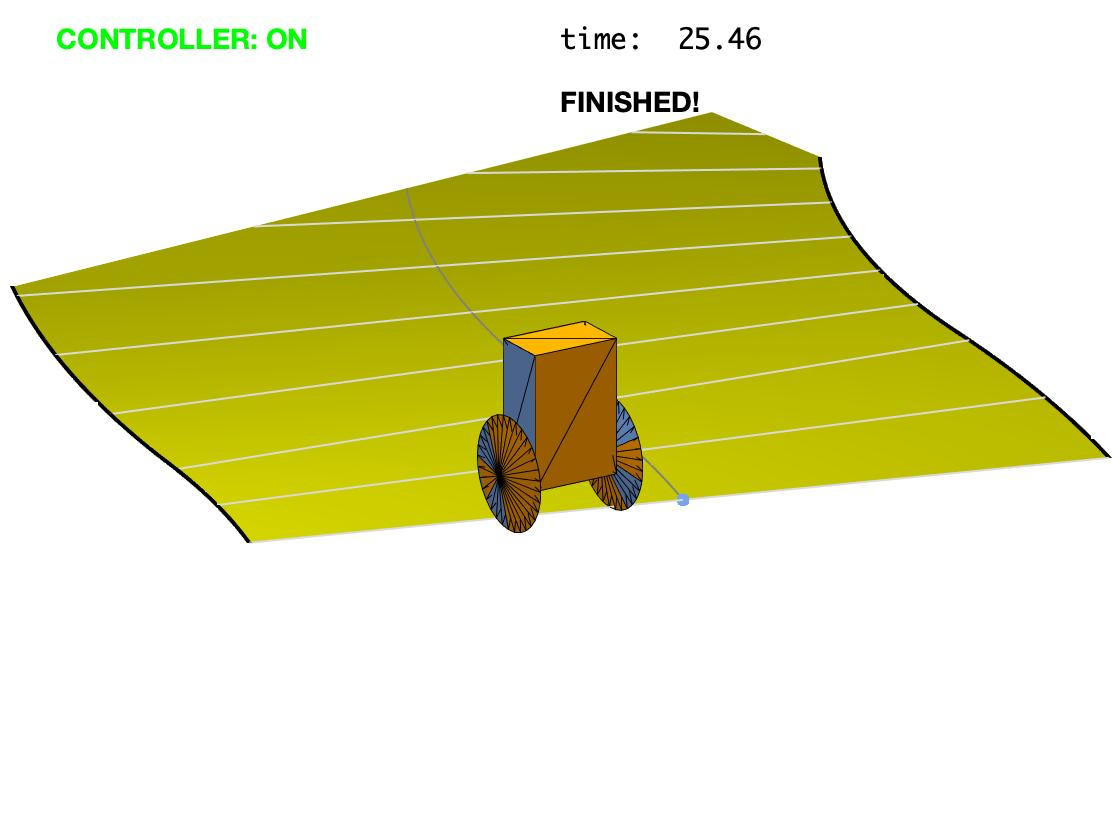
\includegraphics[width=.8\linewidth]{track 2r.jpg}
	\caption{Success 2}
\end{minipage}
\end{figure}
\begin{figure}[H]
\centering
\begin{minipage}{.5\textwidth}
	\centering
	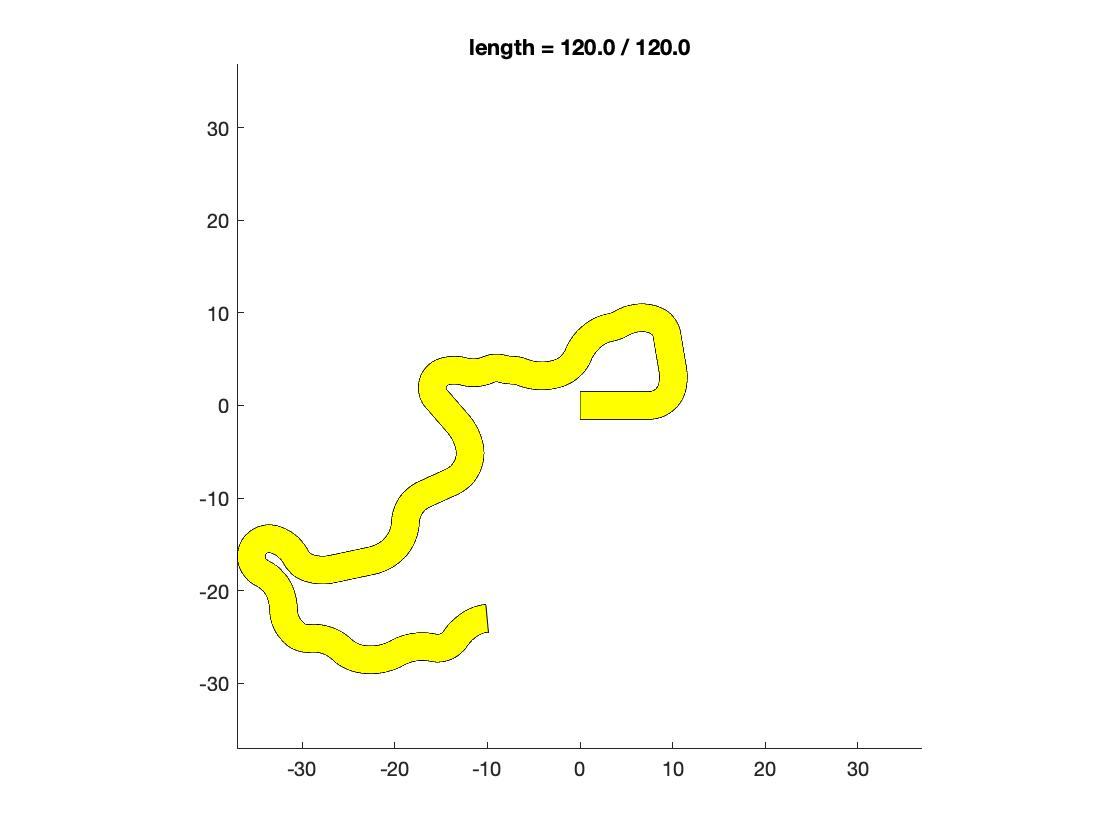
\includegraphics[width=.8\linewidth]{track 3.jpg}
	\caption{Track 3}
	\end{minipage}%
\begin{minipage}{.5\textwidth}
	\centering
	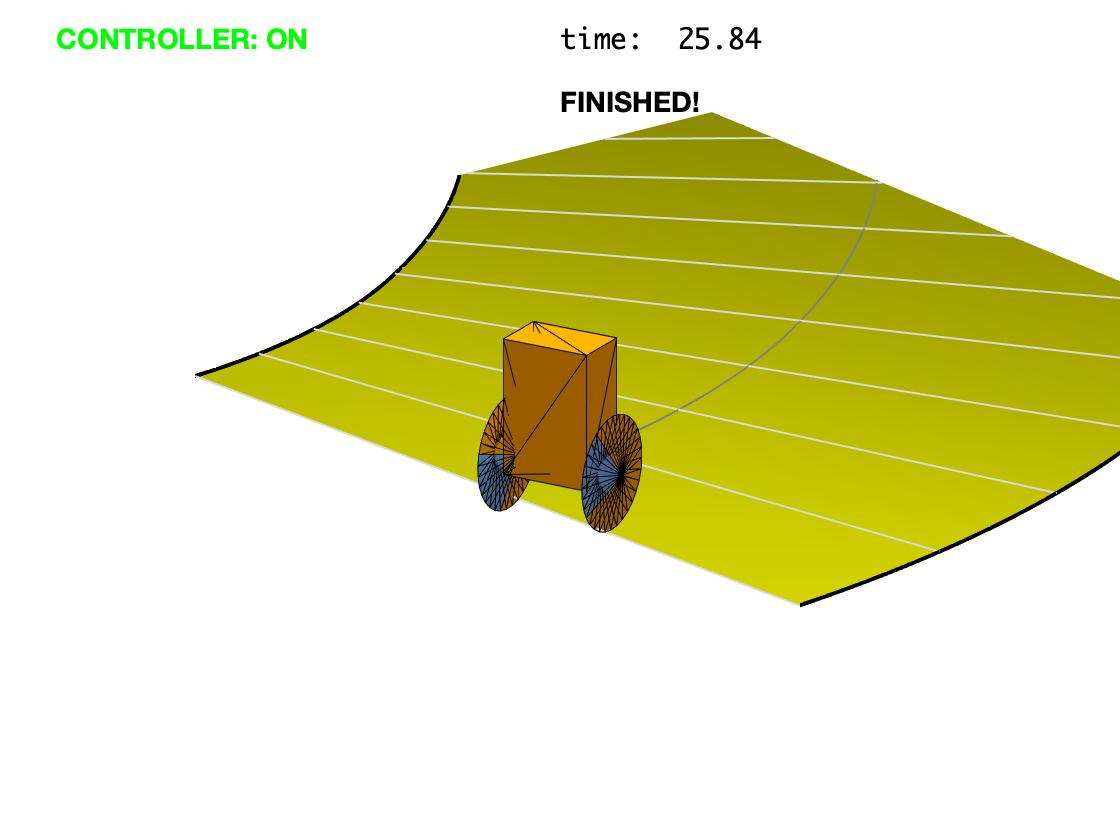
\includegraphics[width=.8\linewidth]{track 3r.jpg}
	\caption{Success 3}
\end{minipage}
\end{figure}
\begin{figure}[H]
\centering
\begin{minipage}{.5\textwidth}
	\centering
	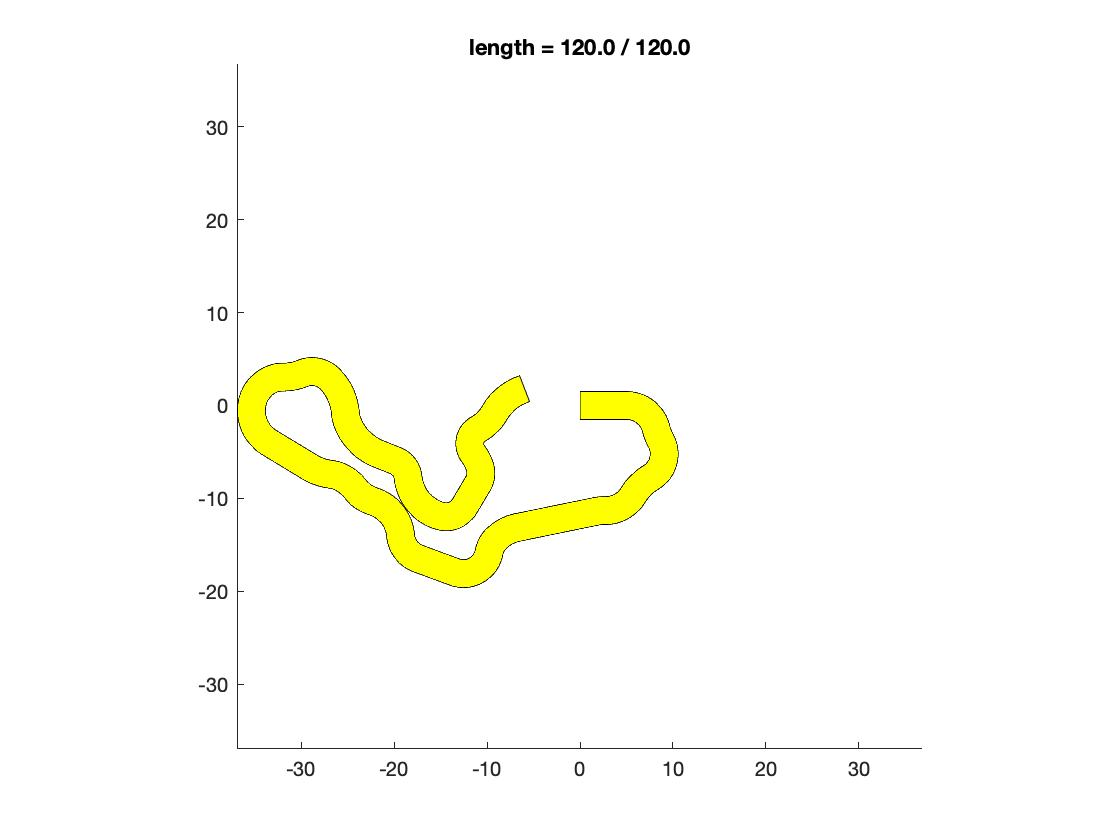
\includegraphics[width=.8\linewidth]{track 4.jpg}
	\caption{Track 4}
	\end{minipage}%
\begin{minipage}{.5\textwidth}
	\centering
	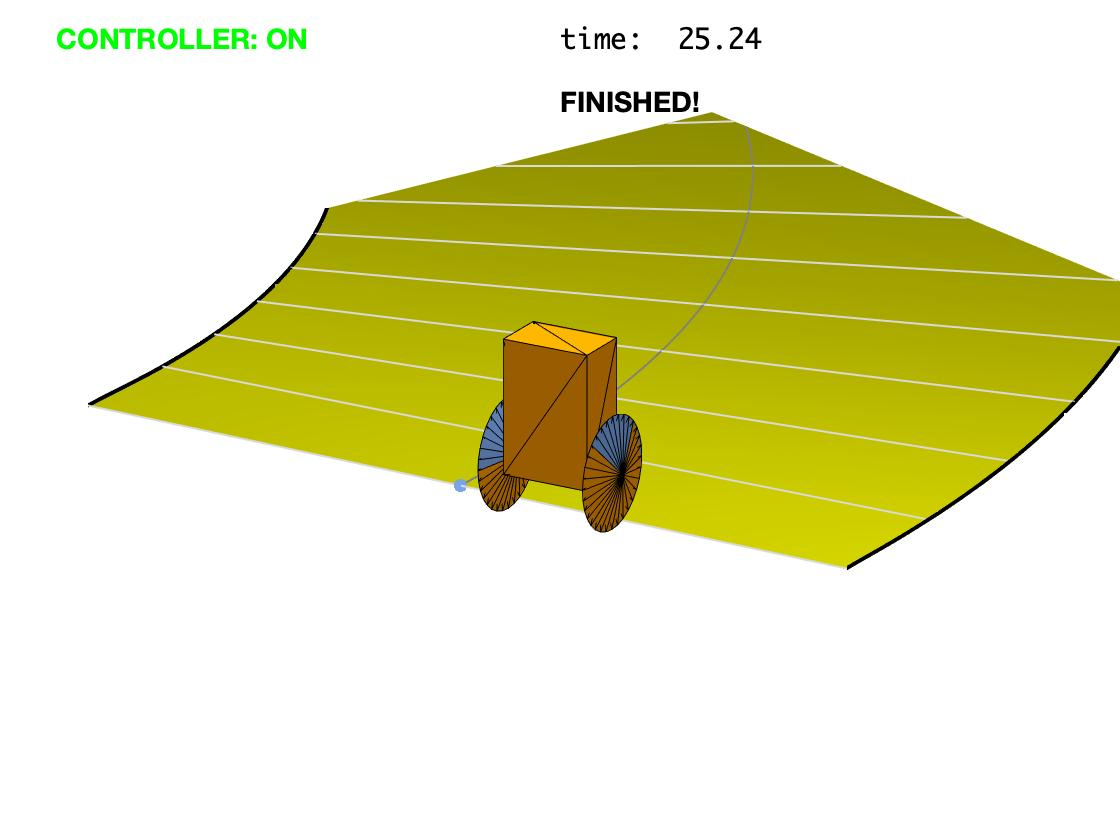
\includegraphics[width=.8\linewidth]{track 4r.jpg}
	\caption{Success 4}
\end{minipage}
\end{figure}
\begin{figure}[H]
\centering
\begin{minipage}{.5\textwidth}
	\centering
	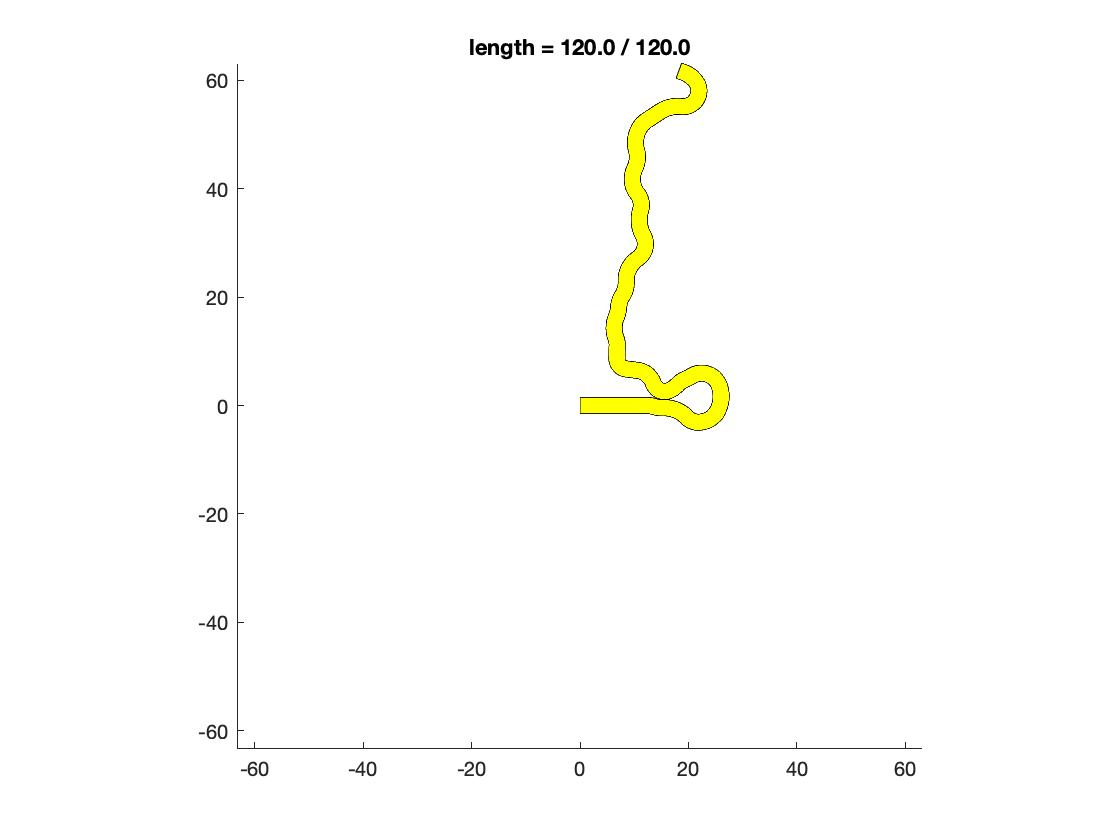
\includegraphics[width=.8\linewidth]{track 5.jpg}
	\caption{Track 5}
	\end{minipage}%
\begin{minipage}{.5\textwidth}
	\centering
	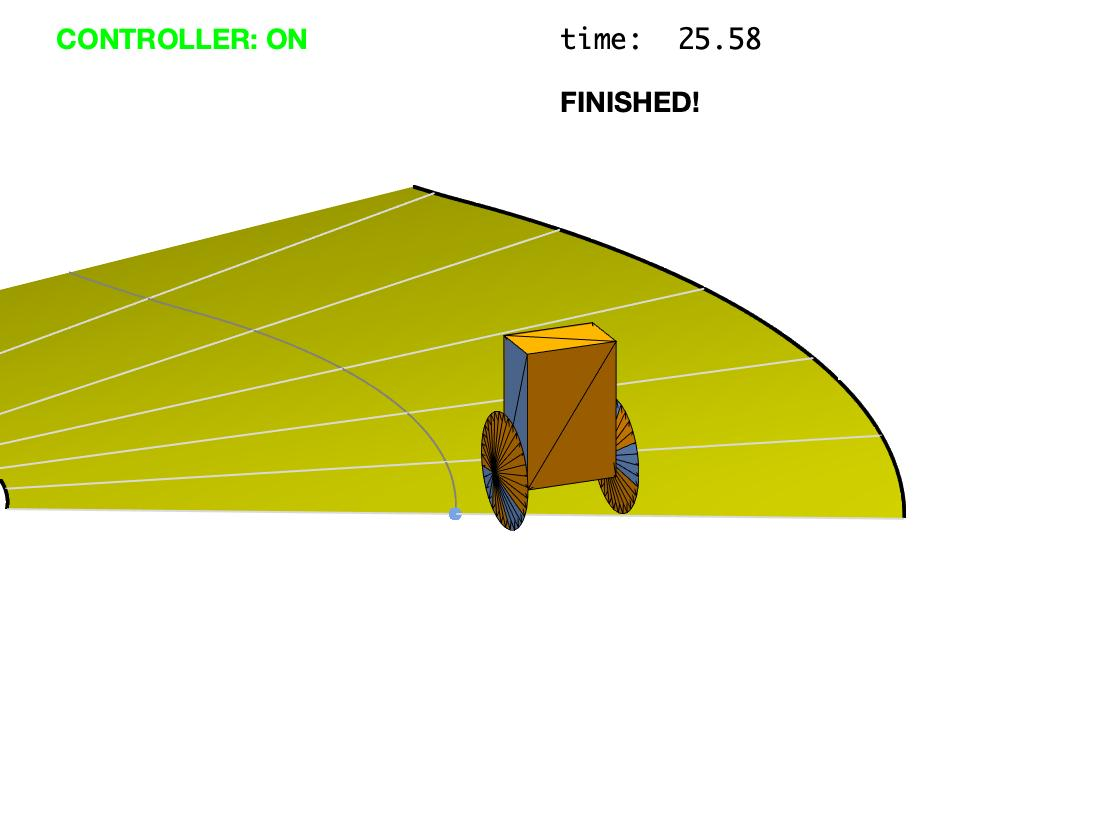
\includegraphics[width=.8\linewidth]{track 5 r.jpg}
	\caption{Success 5}
\end{minipage}
\end{figure}
Therefore, I managed to achieve a 100 $\%$ success rate, but there is obviously chance for failure in some tracks, which can not be accounted for, and that is shown below. We see that my controller crashed early on in this race, which was kind of a let down after 9 consecutive successful runs, but it happens. Not everything can be perfect, and that was shown to me in my 10th trial. Therefore, I can conclusively say that my requirements were fulfilled, where my controller successfully completed 5 consecutive random trials. We could have no failures with the controller present if we slowed it down, but then there would be no point in racing it, thus the controller speed is not reduced from 5.8 m/s. The controller was tested with an equilibrium velocity of 4.5 m/s and never failed, but it averaged 30s per track, which is too slow. The 10th track failure is shown below:
\begin{figure}[H]
\centering
\begin{minipage}{.5\textwidth}
	\centering
	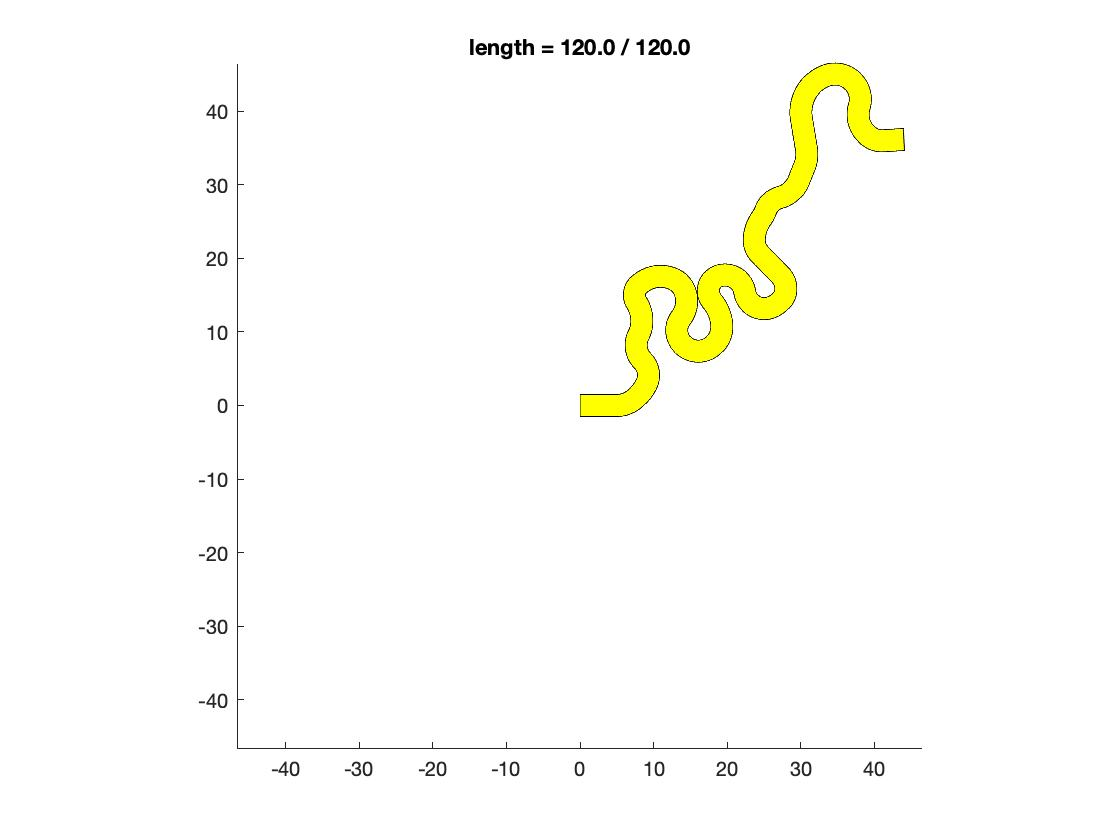
\includegraphics[width=.8\linewidth]{failure.jpg}
	\caption{Track 10}
	\end{minipage}%
\begin{minipage}{.5\textwidth}
	\centering
	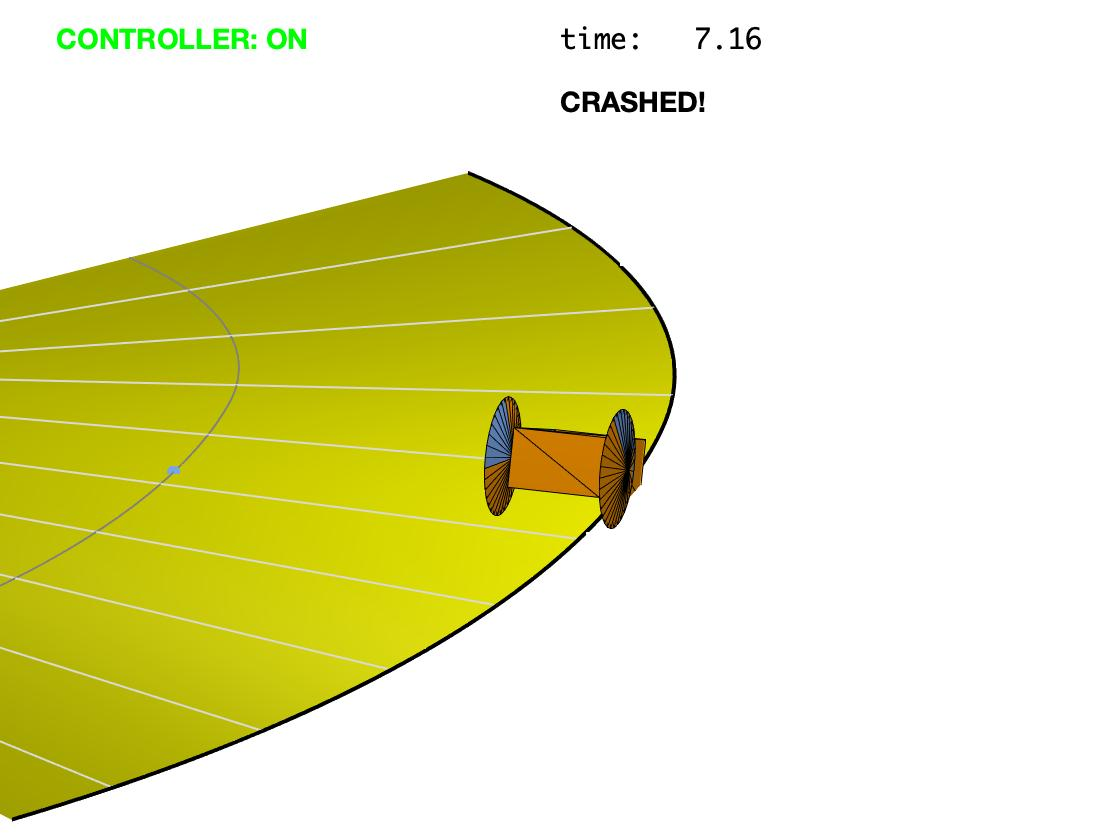
\includegraphics[width=.8\linewidth]{failurer.jpg}
	\caption{Failure}
\end{minipage}
\end{figure}
The robonaut crashed whilst taking sharp and then wide radius turns, showing us the limitations to the controller when increasing speed above a certain limit. Therefore, this is the final gains that I use.
\section{Results}
Each controller behaved differently, but we know that controller 1 was the least effective one. Controller 2 and 3 were similar in success rate, where both crashed in some instanced, but controller 3 was successful more frequently and averaged a lower time. This was to be expected as controller 2 was a dampened version, where it was penalizing its variables much less than controller 3; meaning that it took wider turns, was travelling at a lower speed, and was consistently near the edge of the road.\\
Therefore, from the testing shown above, we can conclude that controller 3 was the most efficient and effective controller produced, with an average of about 25.5 s per race, and a 80$\%$ success rate. What I realized with controller 3 was that it tipped if there were curves as soon as the road started because it was still stabilizing out, however, once it straightened out, regardless of the number of curves and sharp turns, the controller would successfully complete the race. If the speed of the controller was reduced, the success rate increased to nearly 100$\%$ success, however, it was slower than 25.5s, thus I did not reduce my $v_{road}$ and left my controller at 80$\%$ success. I tested this out by running controller 3 through 100 randomly generated races, and the controller successfully completed 83 races out of those 100 races, successfully verifying my requirements. When I reduced equilibrium $v_{road}$ to 4.5 m/s, the controller was able to complete 97 tracks successfully out of a 100, which shows how speed affects the success rate as well.

\section{References}
% Display list of references in IEEE format.
\bibliographystyle{IEEEtran}
\bibliography{IEEEabrv,references}
\end{document}
